\byline{Театърът – начин на живот}{Катерина Карамихалева и Лалита Иванова}

\begin{center}
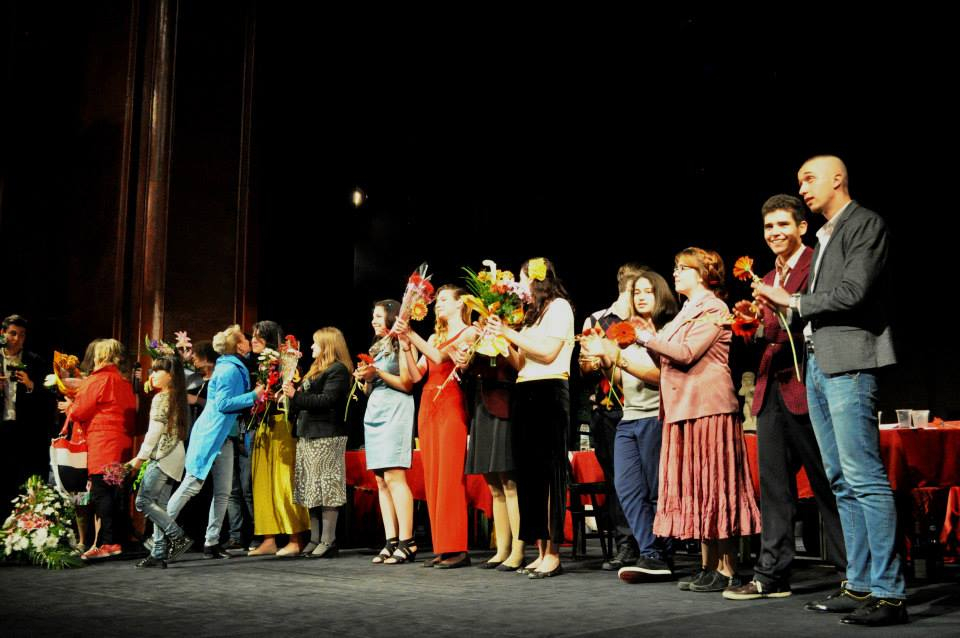
\includegraphics[width=6.2in]{./Teatar/1.jpg}\\
\textit{„Филмите ще те направят известен, телевизията ще те направи богат, но ТЕАТЪРЪТ ще те направи добър.``}
\end{center}

Ние, учениците в Немска езикова гимназия, град Бургас, се стремим да сме част от театъра и неговата магия. Доказателство за този стремеж е именно Театралната трупа на гимназията. В продължение на 55 години театърът е част от ежедневието на учениците и учителите в ГПНЕ „Гьоте“. През 2001-2002г. госпожа Софка Бубалова и нейните ученици полагат основите на трупата с постановките ”Натан мъдреца” и „Добрия човек от Сечуан”. 

Трупата изнася представления ежегодно на сцената на ДТ „Адриана Будевска“, приятелството и подкрепата на бургаския театър са изключително ценни за развитието на младите актьори. Нейни бивши възпитаници са  вече утвърдени имена на сцената – Илиана Коджабашева, Никола Парашкевов, Екатерина Георгиева.

През годините Театрална трупа „Гьоте“ увеличава успехите си все повече. Пиеси от Елин Рахнев,  Камен Донев, Драгомир Асенов, Юра Зойфер и дори сценарии на ученици са представяни на сцена. През 2014г. актьорите печелят трето място на театрален фестивал в Габрово за участието си с пиесата “Schule - deine Zukunft”. Нашето следващо представление очаквайте на 16 април. Насладете се на „Сако от велур“ от Станислав Стратиев!

\newpage
\begin{multicols}{2}

\textbf{Театърът е нашият живот!}

\textit{„Театралната трупа на Немската гимназия беше решаващото, което ме накара да вляза в това училище. Неочаквано там срещнах страхотни хора с много талант, забавна компания, която за няколко часа успява да ме откъсне от сивото ежедневие. Това е изцяло ново преживяване, което не мога да опиша: театралния дух, който те кара да излизаш от кожата си и да влизаш в нечия друга, да общуваш с хората, които познаваш, но те са тотално различни личности. Да се надигравате, да предизвиквате различни ситуации, дори и извън пиесата, за да предизвикате способностите си. Това е нещо друго.“} – Андрея Попова, 12 „Е“ клас \\

\textit{„Театралната трупа преобърна моя живот,чрез нея открих таланта си и моята цел. Винаги ще съм благодарна на ръководителката г-жа Бубалова,че ме научи на всеотдайност и предаде пламъка нататък. Обещавам и аз да го предавам на други!“} – Антоанета Николова,12 „Г“ клас \\

\textit{„Театралната не е просто поредния клуб, в който група деца губят дружно времето си. Там се сблъскваме с много разногласия, различия и проблеми, но се опитваме заедно да ги преодолеем. Учим се как. Учим се и един от друг. Различни сме. По характер, по начин на мислене и по много други неща. С всяка една пиеса, която разиграваме, ние растем. Променяме се, откриваме, вярваме. Вярваме в себе си, в другите, в самата идея. Театърът е като семейството. Изграден е на подкрепа, обич и доверие. Той ме научи да бъда смела, да бъда част от колектив и да си позволя да бъда себе си, макар и играейки чужда роля!“} – Валентина Димова, 12 „Д“ клас \\

\textit{„Трупата е моето второ семейство. Ние сме приятели, колектив и сме едно цяло, когато сме на сцена. Събра ни обичта към театралното изкуство. Театърът ме кара да се чувствам жив, да се въплащавам в различни роли е най-голямото предизвикателство за мен.“} – Георги Колев, 12 „В“ клас \\

\textit{„Театърът е моята най-голяма тръпка, моята най-голяма любов. Там, в театъра, се чувствам жива, щастлива, истинска. Театралната трупа ми помогна да се чувствам така всеки ден, играейки различни роли, обичайки всяка една от тях. Научих се на увереност, отговорност... Намерих приятели за цял живот. Но най-важното: станах част от най-красивото изкуство.“} – Катерина Карамихалева, 12 „Б“ клас \\

\textit{„Понякога почивка от сивото ежедневие е нещото, от което всеки има нужда. Театърът е моето бягство. За мен най-голямото удоволствие е да вляза в поредната колоритна роля, независимо била тя млада, възрастна или дори мъжка. А театралната трупа като всяко друго извънучебно занятие ни учи на дисциплина, работа в екип, сплотеност.. Запознаваш се с хора с различни интереси и виждания за нещата, сключваш нови и интересни приятелства.“} – Лалита Иванова, 12 „Д“ клас \\

\textit{„Главната причина да вляза в гимназията бе точно театралната трупа. Бях присъствала на представления и ентусиазмът на учениците ме подтикна да избера театъра, като занимание в свободното ми време. Когатостанах част от тфупата разбрах колко труд и усилия са нужни докато се постигне крайния резултат. Участието в трупата ме научи на отговорност, защото там не си сам, а всички сте един екип. Освен това по време на репетициите се сближаваш с другите театрали и заедно имате много радостни моменти.“} – Калина Кърпичева,11 „В“ клас \\

\textit{„Театърът ми  дава всичко, което ми е необходимо, и с нищо не ме ограбва. приемам го като мое призвание, защото  не възприема театъра като работа, а по-скоро като едно огромно удоволствие. Времето прекарано със съученици ми от 10, 11 и 12 клас не може да се замени с нищо. Часове, в който има както и доза смях така и сериозност. Двете най важни неща на който ме учи театърът е да поемам отговорност за действията си и съответно за последствията, и съща така да намирам балансът. Той е най - важен.“} – Делян Петков,10 „В“клас \\

\textit{„Част от групата съм, защото театърът е едно голямо семейство! Кара ме да се чувствам щастлива, различна, разбрана. Чрез него се научих да изразявам чувствата си чрез думи, чрез игра, дори и чрез поглед. Научих се да бъда търпелива, да се трудя и старая, научих се и да не се отказвам. Театърът е нещото, от което всеки се нуждае, дори и за просто малко разнообразие.“} – Елена Янева,10 „В“ клас \\

\textit{„Аз лично се включих в театралната група на гимназията защото ми допада театралното изкуство и защото ми харесва да се запознавам с нови хора, и не съжалявам че го направих. Тя ми показа, че дори една  група от най-различни хора може да има една цел и да я осъществи.“ } – Иван Стоянов, 10 „Д“ клас

\closearticle
\end{multicols}


